\begin{Exercise}[title=Intérférences ultrasonores]
  Une expérience d’interférences d’ondes ultrasonores est réalisée. La fréquence d’émission
est égale à $40 kHz$ , ce qui correspond à une longueur d’onde$\lambda = 8,5 mm$. Sauf à la question
3. Les sources $E_1$ et $E_2$ émettent des ondes acoustiques en phase. On note $O$ le point milieu du segment délimité par les émetteurs distant de $a = 4 cm$ et Ox l’axe situé sur la médiatrice de ce segment. On déplace le microphone sur un grand cercle de
rayon $R = 0,5 m$ et on relève l’évolution de l’amplitude mesurée en fonction de l’angle $\theta$ que la direction $OM$ avec l’axe $Ox$.
\Question Distance d'interfrange
\subQuestion Faire une figure faisant apparaitre les points $O$, $E_1$ et$ E_2$ et $M$ pour un
angle $\theta$ non nul, $M$ étant situé du même côté de la bissectrice $Ox$ que le point $E_2$ .
\subQuestion Tracer l’arc de cercle de centre $M$ passant par $E_2$ , on note $H$ son
intersection avec la droite $E_1 M$. Que représente $E_1 H$ ?
\subQuestion Puisque $R \gg a$, on peut assimiler $H$ et le projeté de $E_2$ sur $E_1 M$. En
déduire une expression du déphasage entre les ondes reçues en $M$ en
fonction de$\theta, a$ et $\lambda$.
\subQuestion Quelles sont, dans l’intervalle $[-30^o, 30^o]$ , les valeurs de $\theta$ où on
observe un maximum d’amplitude résultante ?
\Question Minima d'amplitude
\subQuestion Sur l’intervalle d’étude précédent, quelles sont les positions où un
minimum d’amplitude est attendu ?
\subQuestion Si les ondes reçues ont la même amplitude, quelle valeur d’amplitude
minimale est prévue par la théorie ?
\Question inversion de phase

Le dispositif permet d’inverser le signal émis par l’un des émetteurs (ce qui
revient à le déphaser de $\pi$.
\subQuestion Quel est l’état d’interférences sur l’axe Ox ?
\subQuestion Quelles sont les positions des nouveaux points de maximum et de
minimum d’amplitude ?
\subQuestion Qu’advient-il si l’on inverse également l’autre signal ?
\end{Exercise}
\begin{Answer}
  \Question
  \subQuestion
  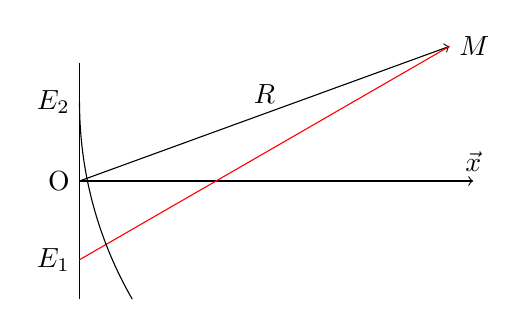
\begin{tikzpicture}
    \draw[->](0,0)node[left]{O} -- (5,0) node[above]{$\vec{x}$};
    \draw (0,-1.5) -- (0,-1)node(E1){} node[left]{$E_1$} -- (0,1)node(E2){} node[left]{$E_2$} -- (0,1.5);
    \draw[->] (0,0)  -- ++(20:5) node(M){} node[midway, above]{$R$} node[above,right]{$M$};
    \draw[red] (20:5) -- (0,-1);
    \draw (0,1) arc (180:210:5);

  \end{tikzpicture}
\subQuestion
$E_1H$ est la différence $E_1M - E_2M = r_2 - r_1$ c’est la différence de
distances parcourues par les 2 ondes acoustiques.
\subQuestion
En raisonnant dans le triangle quasiment rectangle $E_1 E_2 H$, on obtient
$E_1 H \simeq asin \theta$. On en déduit donc le déphasage : $\phi=\frac{2\pi asin\theta}{\lambda}$
\subQuestion
Les interférences constructives sont obtenues lorsque $\phi$ est un $p\lambda$
multiple de $2\pi$. On a $\sin \theta =\frac{p\lambda}{a}$ avec $p$ entier.
Pour $p = 0$, ie sur l’axe Ox, un maximum d’amplitude est observé.
(Symétries)
Pour $p = \pm 1$, l’angle $\theta = \pm12^o$
Pour $p = \pm 2$, l’angle $\theta = \pm 25^o$ ce qui environ le double de la valeur
précédente.
Pour les ordres plus élevées de l’ordre $p$ ne sont pas dans l’intervalle
proposé.
\Question
\subQuestion
L’interférences destructives sont obtenues lors d’une opposition de
phase des ondes $\phi = \pi + 2p\pi$. Il s’agit de $\phi = \pm \pi$ donc $\theta = \pm 6^o$ et
$\phi = \pm 3\pi$ donc $\theta = \pm 19^o$.
\subQuestion Pour des ondes reçues avec la même amplitude, l’opposition de phase
doit conduire à une annulation de l’amplitude résultante.
\Question
\subQuestion
Sur l’axe Ox, les durées de trajet des ondes sont identiques, donc le
déphasage est égal à celui de l’émission. Les ondes reçues sont donc en
opposition de phase : les interférences sont destructives.
\subQuestion Ajouter $\pi$ au déphasage $\phi$ revient à intervertir les lieux de maximum
et de minimum d’amplitude.
\subQuestion Inverser l’autre signal revient à rétablir la mise en phase des deux
émissions : on retrouve les observations initiales.

\end{Answer}
